\documentclass[12pt, oneside]{article}

\usepackage{amssymb,amsmath,pifont,amsfonts,comment,enumerate,enumitem}
\usepackage{currfile,xstring,hyperref,tabularx,graphicx,wasysym}
\usepackage[labelformat=empty]{caption}
\usepackage[dvipsnames,table]{xcolor}
\usepackage{multicol,multirow,array,listings,tabularx,lastpage,textcomp,booktabs}

% NOTE(joe): This environment is credit @pnpo (https://tex.stackexchange.com/a/218450)
\lstnewenvironment{algorithm}[1][] %defines the algorithm listing environment
{   
    \lstset{ %this is the stype
        mathescape=true,
        frame=tB,
        numbers=left, 
        numberstyle=\tiny,
        basicstyle=\rmfamily\scriptsize, 
        keywordstyle=\color{black}\bfseries,
        keywords={,procedure, div, for, to, input, output, return, datatype, function, in, if, else, foreach, while, begin, end, }
        numbers=left,
        xleftmargin=.04\textwidth,
        #1
    }
}
{}
\lstnewenvironment{java}[1][]
{   
    \lstset{
        language=java,
        mathescape=true,
        frame=tB,
        numbers=left, 
        numberstyle=\tiny,
        basicstyle=\ttfamily\scriptsize, 
        keywordstyle=\color{black}\bfseries,
        keywords={, int, double, for, return, if, else, while, }
        numbers=left,
        xleftmargin=.04\textwidth,
        #1
    }
}
{}

\newcommand\abs[1]{\lvert~#1~\rvert}
\newcommand{\st}{\mid}

\newcommand{\A}[0]{\texttt{A}}
\newcommand{\C}[0]{\texttt{C}}
\newcommand{\G}[0]{\texttt{G}}
\newcommand{\U}[0]{\texttt{U}}

\newcommand{\cmark}{\ding{51}}
\newcommand{\xmark}{\ding{55}}



\begin{document}
\begin{flushright}
\StrBefore{\currfilename}{.}
\end{flushright}

\section*{This week's highlights}
\begin{itemize}
\item Evaluate the truth value of a compound proposition given truth values of its constituent variables.
\item Prove propositional equivalences using truth tables
\item Prove propositional equivalences using other known equivalences, e.g.
\begin{itemize}
\item DeMorgan's laws
\item Double negation laws
\item Distributive laws, etc.
\end{itemize}
\item Compute the CNF and DNF of a given compound proposition.
\item Translate sentences from English to propositional logic using appropriate propositional variables and boolean operators.
\item Form the converse, contrapositive, and inverse of a given conditional statement.
\item Decide and justify whether or not a collection of propositions is consistent.
\end{itemize}

\section*{Lecture videos}
Monday: No class in observance of Martin Luther King day.

\href{https://www.youtube.com/watch?v=6KLTpoTpkXo}{A video to reflect on the role of algorithms in
systemic racism. Credit: Safiya Umoja Noble.}

Week 3 Day 1
\href{https://youtube.com/playlist?list=PLML4QilACLk4eQeliamh26adMOwifz8Uj}{YouTube playlist}

Week 3 Day 2
\href{https://youtube.com/playlist?list=PLML4QilACLk7GdezMI_tPsCB2iJ5f7ikp}{YouTube playlist}

\newpage
\section*{Wednesday January 20}

\begin{tabular}{lp{5in}}
{\bf Proposition} & Declarative sentence that is true or false (not both).\\
{\bf Propositional variable} & Variable that represents a proposition.\\
{\bf Compound proposition}& New propositions formed from existing propositions (potentially) using logical operators.\\
{\bf Truth table}& Table with 1 row for each of the possible combinations of truth values of the input and 
an additional column that shows the truth value of the result of the operation corresponding to a particular row.
\end{tabular}

{\it Note}: A propositional variable is one example of a compound proposition.

{\bf Logical operators} aka propositional connectives

\begin{tabular}{lccccp{4in}}
{\bf Conjunction} & AND & $\land$ &\verb|\land| & 2 inputs & Evaluates to $T$ when {\bf both} inputs are $T$\\
{\bf Exclusive or} & XOR & $\oplus$ &\verb|\oplus| & 2 inputs & Evaluates to $T$ when {\bf exactly one} of inputs is $T$\\
{\bf Disjunction} & OR & $\lor$ &\verb|\lor| & 2 inputs & Evaluates to $T$ when {\bf at least one} of inputs is $T$\\
{\bf Negation} & NOT & $\lnot$ &\verb|\lnot| & 1 input & Evaluates to $T$ when its input is $F$\\
\end{tabular}

\begin{center}
\begin{tabular}{cc||c|c|c}
\multicolumn{2}{c||}{Input}  & \multicolumn{3}{c}{Output} \\
 & & {\bf Conjunction} &  {\bf Exclusive or} & {\bf Disjunction} \\
$p$ & $q$ & $p \land q$ &  $p  \oplus  q$ & $p \lor  q$ \\
\hline
$T$ & $T$ & $T$ & $F$ & $T$\\
$T$ & $F$ & $F$ & $T$ & $T$\\
$F$ & $T$ & $F$ & $T$ & $T$\\
$F$ & $F$ & $F$ & $F$ & $F$\\
\end{tabular}
\qquad \qquad\qquad
\begin{tabular}{c||c}
Input & Output \\
 & {\bf Negation} \\
$p$ & $\lnot p$ \\
\hline
$T$ & $F$ \\
$F$ & $T$\\
\end{tabular}
\end{center}

\vfill

\begin{center}
\begin{tabular}{ccc||p{3in}|c|c}
\multicolumn{3}{c||}{Input}  & \multicolumn{3}{c}{Output} \\
$p$ & $q$ & $r$  &  &  $(p \land q) \oplus (~ ( p \oplus q) \land r~)$ & $(p \land q) \vee (~ ( p \oplus q) \land r~)$ \\
\hline
$T$ & $T$  & $T$ &   && \\
$T$ & $T$  & $F$ &   && \\
$T$ & $F$  & $T$ &   && \\
$T$ & $F$  & $F$ &   && \\
$F$ & $T$  & $T$ &   && \\
$F$ & $T$  & $F$ &   && \\
$F$ & $F$  & $T$ &   && \\
$F$ & $F$  & $F$ &   && \\
\end{tabular}
\end{center}
\vfill

\newpage
\begin{tabular}{lp{4in}p{2in}}
{\bf Logical equivalence } &Two compound  propositions are {\bf logically  equivalent} means that  they 
have the  same  truth  values for all settings of truth  values to their propositional  variables.\\
{\bf Tautology} & A compound proposition that evaluates to true
for all settings of truth  values to its propositional  variables; it is  abbreviated $T$.\\
{\bf Contradiction} & A compound proposition that  evaluates  to  false 
for  all settings of truth  values to its propositional  variables; it  is abbreviated $F$.\\
{\bf Contingency} & A compound proposition that is neither a tautology nor a contradiction.\\
\end{tabular}

{\it Extra Example}: Which of the  compound propositions in the table below are logically equivalent?
\begin{center}
\begin{tabular}{cc||c|c|c|c|c}
\multicolumn{2}{c||}{Input}  & \multicolumn{5}{c}{Output} \\
$p$ & $q$ & $\lnot (p \land \lnot q)$ & $\lnot (\lnot p  \lor \lnot q)$ &  $(\lnot p \lor  q)$
& $(\lnot q \lor \lnot p)$ & $(p \land q)$  \\
\hline
$T$ & $T$ & &&&&\\
$T$ & $F$ & &&&&\\
$F$ & $T$ & &&&&\\
$F$ & $F$ & &&&&\\
\end{tabular}
\end{center}


{\bf (Some)} logical equivalences) cf. Rosen pp. 26-28

\begin{tabular}{llp{3in}}
$p \lor q \equiv q \lor p$ & $p \land q \equiv q \land p$ & {\bf Commutativity} Ordering of terms\\
$(p \lor q) \lor r  \equiv p \lor (q \lor r)$ & $(p \land q) \land r  \equiv p \land (q \land r)$ & {\bf Associativity} Grouping of terms\\
$p \land F \equiv F$ \qquad $p \lor T \equiv T$ & $p \land T \equiv p$ \qquad $p \lor F \equiv p$ & {\bf Absorption} aka 
short circuit evaluation\\
$\lnot (p \land q) \equiv \lnot p \lor \lnot q$ & $\lnot (p \lor q) \equiv \lnot p \land\lnot q$  & {\bf DeMorgan's Laws}\end{tabular}


{\it Can replace $p$ and $q$ with any compound proposition}

\vfill

\newpage
Given an compound proposition, we can use
\begin{itemize}
\item Truth tables
\item Logical equivalences
\end{itemize}
to compute its truth value for specific input values.

Now, given a truth table, how do we find a compound proposition that has the specified output values?

{\it Application}: design a circuit given a desired input-output relationship.

\begin{center}
\begin{tabular}{cc||cc}
\multicolumn{2}{c||}{Input}  &\multicolumn{2}{c}{Output}\\
$p$ & $q$& $mystery_1$ & $mystery_2$\\
\hline
$T$ & $T$  & $T$ & $F$\\
$T$ & $F$  & $T$ & $F$\\
$F$ & $T$  & $F$ & $F$\\
$F$ & $F$  & $T$ & $T$\\
\end{tabular}
\qquad \qquad
\begin{tabular}{ccc||c}
\multicolumn{3}{c||}{Input}  & Output\\
$p$ & $q$ & $r$  &  ?\\
\hline
$T$ & $T$  & $T$ & $T$ \\
$T$ & $T$  & $F$ & $T$ \\
$T$ & $F$  & $T$ & $F$ \\
$T$ & $F$  & $F$ & $T$ \\
$F$ & $T$  & $T$ & $F$ \\
$F$ & $T$  & $F$ & $F$ \\
$F$ & $F$  & $T$ & $T$ \\
$F$ & $F$  & $F$ & $F$ \\
\end{tabular}

\end{center}


A compound proposition that  gives output $mystery_1$ is: \underline{\phantom{\hspace{3in}}}


\vfill


A compound proposition that  gives output $mystery_2$ is: \underline{\phantom{\hspace{3in}}}


\vfill



{\bf  Definition} A compound proposition is in {\bf disjunctive normal form}  (DNF) means
that  it is an OR of ANDs of variables and their negations.

{\bf  Definition} A compound proposition is in {\bf conjunctive normal form}  (CNF) means
that  it is an AND of ORs of variables and their negations.


{\it Extra example}: A compound proposition that  gives output ? is: 


\vfill
\vfill

\newpage
\section*{Friday January 22}

The only way to make  the conditional statement $p \to q$ false is to \underline{\phantom{\hspace{3in}}}


\begin{tabular}{llll}
The {\bf  hypothesis}  of $p \to q$ is  &\underline{\phantom{\hspace{1in}}} &
The {\bf  antecedent}  of $p \to q$ is  &\underline{\phantom{\hspace{1in}}} \\
&&&  \\
The {\bf  conclusion}  of $p \to q$ is & \underline{\phantom{\hspace{1in}}}&
The {\bf  consequent}  of $p \to q$ is & \underline{\phantom{\hspace{1in}}}\\
&&&  \\
\end{tabular}

\vfill

\begin{center}
\begin{tabular}{cc||c|c|c|c|c}
\multicolumn{2}{c||}{Input}  & \multicolumn{5}{c}{Output} \\
 & & Conjunction &  Exclusive or & Disjunction  &  Conditional & Biconditional  \\
$p$ & $q$ & $p \wedge q$ &  $p  \oplus  q$ & $p \vee  q$ & $p \to q$ & $p \leftrightarrow q$\\
\hline
$T$ & $T$ & $T$ & $F$ & $T$ & $T$& $T$\\
$T$ & $F$ & $F$ & $T$ & $T$ & $F$& $F$\\
$F$ & $T$ & $F$ & $T$ & $T$ & $T$& $F$\\
$F$ & $F$ & $F$ & $F$ & $F$ & $T$& $T$\\
\end{tabular}
\end{center}

{\it Examples} 

$p \to q \equiv \lnot p \lor q$ because \underline{\phantom{\hspace{4in}}} 

\vfill

$p \leftrightarrow q$ is not logically equivalent to $p \land q$ because \underline{\phantom{\hspace{4in}}} 

\vfill

$\lnot( p \leftrightarrow q) \equiv p \oplus q$ because \underline{\phantom{\hspace{4in}}} 

\vfill


$p \to q$ is not logically equivalent to $q \to p$ because \underline{\phantom{\hspace{4in}}} 

\vfill

$p \leftrightarrow q \equiv q \leftrightarrow p$ because \underline{\phantom{\hspace{4in}}} 

\vfill

\begin{tabular}{ll}
The {\bf  converse}  of $p \to q$ is & \underline{\phantom{\hspace{1.6in}}}\\
&  \\
The {\bf  inverse}  of $p \to q$ is  &\underline{\phantom{\hspace{1.6in}}}\\
&  \\
The {\bf  contrapositive}  of $p \to q$ is & \underline{\phantom{\hspace{1.6in}}}
\end{tabular}
Which of these is logically equivalent to $p \to q$?

\vfill
\vfill

\newpage
{\bf Translation}: Express each of the following sentences as compound propositions, using
the given propositions.

\begin{multicols}{2}
``A sufficient condition for the warranty to be good is that you bought the computer less than a year ago"
\columnbreak
\begin{align*}
w &\text{ is  ``the warranty is good"} \\
b &\text{ is  ``you bought the computer less than a year ago"} \\
\end{align*}
\end{multicols}
\vfill

\begin{multicols}{2}
``Whenever the message was sent from an unknown system, it is scanned for viruses."
\columnbreak
\begin{align*}
s &\text{ is  ``The message is scanned for viruses"} \\
u &\text{ is  ``The message was sent from an unknown system"} \\
\end{align*}
\end{multicols}
\vfill

\begin{multicols}{2}
``I will complete my to-do list only if I put a reminder in my calendar"
\columnbreak
\begin{align*}
r &\text{ is  ``I will complete my to-do list"} \\
c &\text{ is  ``I put a reminder in my calendar"} \\
\end{align*}
\end{multicols}
\vfill


\section*{Review quiz questions}
\begin{enumerate}
\item {\bf Wednesday}
\begin{enumerate}
\item Consider the logic circuit
    \begin{center}
    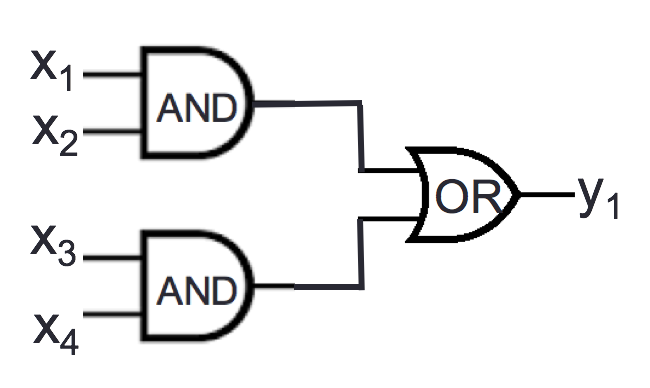
\includegraphics[width=2in]{../resources/images/review-circuit-3.png}
    \end{center}
    For which of the following settings(s) of input values is the output
    $y_1 =  0$? (Select all and only those that apply.)
    \begin{enumerate}
        \item $x_1 = 0$, $x_2 = 0$, $x_3 = 0$, and $x_4 = 0$
        \item $x_1 = 1$, $x_2 = 1$, $x_3 = 1$, and $x_4 = 1$
        \item $x_1 = 1$, $x_2 = 0$, $x_3 = 0$, and $x_4 = 1$
        \item $x_1 = 0$, $x_2 = 0$, $x_3 = 1$, and $x_4 = 1$
    \end{enumerate}
\item Consider the logic circuits
    \begin{center}
    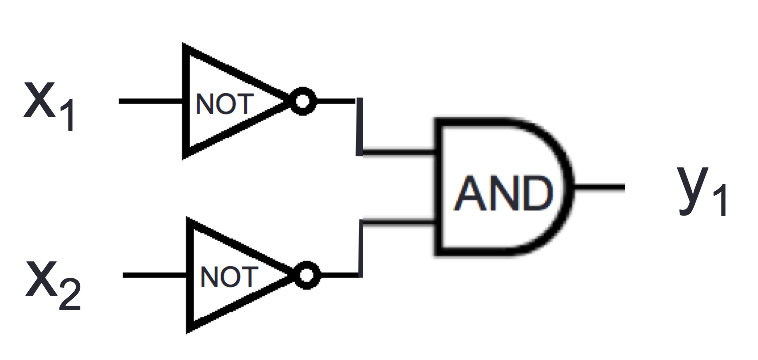
\includegraphics[width=2in]{../resources/images/review-circuit-1.png}
    \qquad \qquad \qquad
    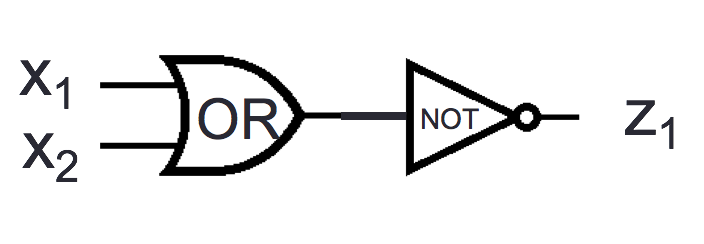
\includegraphics[width=2in]{../resources/images/review-circuit-4.png}
    \end{center}
    For which  of the following settings(s) of input values do the outputs
    of these  circuits have the  same value, i.e.\ $y_1 =  z_1$? 
    (Select all and only those that apply.)
    \begin{enumerate}
        \item $x_1 = 1$, $x_2 = 1$
        \item $x_1 = 1$, $x_2 = 0$
        \item $x_1 = 0$, $x_2 = 1$
        \item $x_1 = 0$, $x_2 = 0$
    \end{enumerate}    
    
\end{enumerate}

\item {\bf Wednesday} For each of the following propositions, indicate exactly one of:

\begin{itemize}
    \item There is no assignment of truth values to its variables that makes it true,
    \item There is exactly one assignment of truth values to its variables that makes it true, or
    \item There are exactly two assignments of truth values to its variables that make it true, or
    \item There are exactly three assignments of truth values to its variables that make it true, or
    \item \emph{All} assignments of truth values to its variables make it true.
\end{itemize}

\begin{enumerate}
    \item $x \land y \land (x \lor y)$
    \item $\lnot x \land y \land (x \lor y)$
    \item $x \land \lnot y \land (x \land y)$
    \item $\lnot x \land (y \lor \lnot y)$
    \item $x \land (y \lor \lnot x)$
\end{enumerate}

\newpage
\item {\bf Friday} For each of the following propositions, indicate exactly one of:

\begin{itemize}
    \item There is no assignment of truth values to its variables that makes it true,
    \item There is exactly one assignment of truth values to its variables that makes it true, or
    \item There are exactly two assignments of truth values to its variables that make it true, or
    \item There are exactly three assignments of truth values to its variables that make it true, or
    \item \emph{All} assignments of truth values to its variables make it true.
\end{itemize}

\begin{enumerate}
    \item $(p \leftrightarrow q) \oplus (p \land q)$
    \item $(p \to q) \vee (q \to p)$
    \item $(p \to q) \land (q \to p)$
    \item $\lnot (p \to q) $
\end{enumerate}
\item {\bf Friday} {\bf Definition}: A collection of  compound  propositions
is called {\bf consistent} if  there
is  an assignment  of  truth values
to  the  propositional variables that makes
each of the compound propositions  true.

For each of  the following  system specifications, 
identify the compound propositions  that give their
translations to logic  and then determine if the
translated collection  of compound
propositions is consistent.

\begin{enumerate}
    \item Specification: If the computer is out of memory, then network connectivity is unreliable. No disk errors can occur when the computer is out of memory. Disk
    errors only occur when network connectivity is unreliable.
    
    Translation: $M =$ ``the computer is  out of memory"; $N = $ ``network connectivity
    is unreliable"; $D = $  ``disk errors  can occur".
    
    \begin{enumerate}
        \item \begin{align*} &\neg M \to  N  \\ & \neg D \to M \\ & D \to N \end{align*}
        \item \begin{align*} &M \to  \neg N  \\ & \neg D \wedge M \\ & N \to D \end{align*}
        \item \begin{align*} &M \to  N  \\ &  M \to \neg D \\ & \neg  N \to \neg D \end{align*}
    \end{enumerate}
    
    \newpage
    \item Specification: Whether you think you can, or you think you can't - you're right.
\footnote{Henry Ford}
    
    Translation: $T =$ ``you  think  you  can"; $C = $  ``you  can".
    
    \begin{enumerate}
        \item \begin{align*} &T \to C \\&  \neg T \to \neg C \end{align*}
        \item \begin{align*} &T \wedge C \\  & \neg  T \wedge \neg C \end{align*}
        \item \begin{align*} &T \to \neg T  \\ & C  \to \neg  C \end{align*}
    \end{enumerate}
    
    \item Specification: A secure password must be private and complicated. If
    a password is  complicated then  it will be hard to  remember.  People
    write down hard-to-remember passwords. If a password is written down, it's  not private.   The password is secure.

    Translation: $S =$ ``the password is secure"; $P = $ ``the password is private"; 
    $C = $  ``the password is  complicated"; $H = $ ``the password is hard to remember";
    $W =  $ ``the password is written down".
    
    \begin{enumerate}
        \item \begin{align*} &\neg (P \wedge C) \to \neg  S  \\ & C \to H  \\ & W \wedge H \\ & W \to  \neg P \\ & S \end{align*}
        \item \begin{align*} &(P \wedge  C)  \to S  \\ &  C \to H\\ & W  \to  H \\  & W \to P \\ & S\end{align*}
        \item \begin{align*} & S  \to (P \wedge C)  \\ &  C \to H\\ & H  \to  W \\  & W \to \neg P \\ & S\end{align*}
\end{enumerate}

\end{enumerate}
\end{enumerate}
\end{document}
